\section{実験設計\label{approach}}
  \begin{figure*}[t]
    \centering
    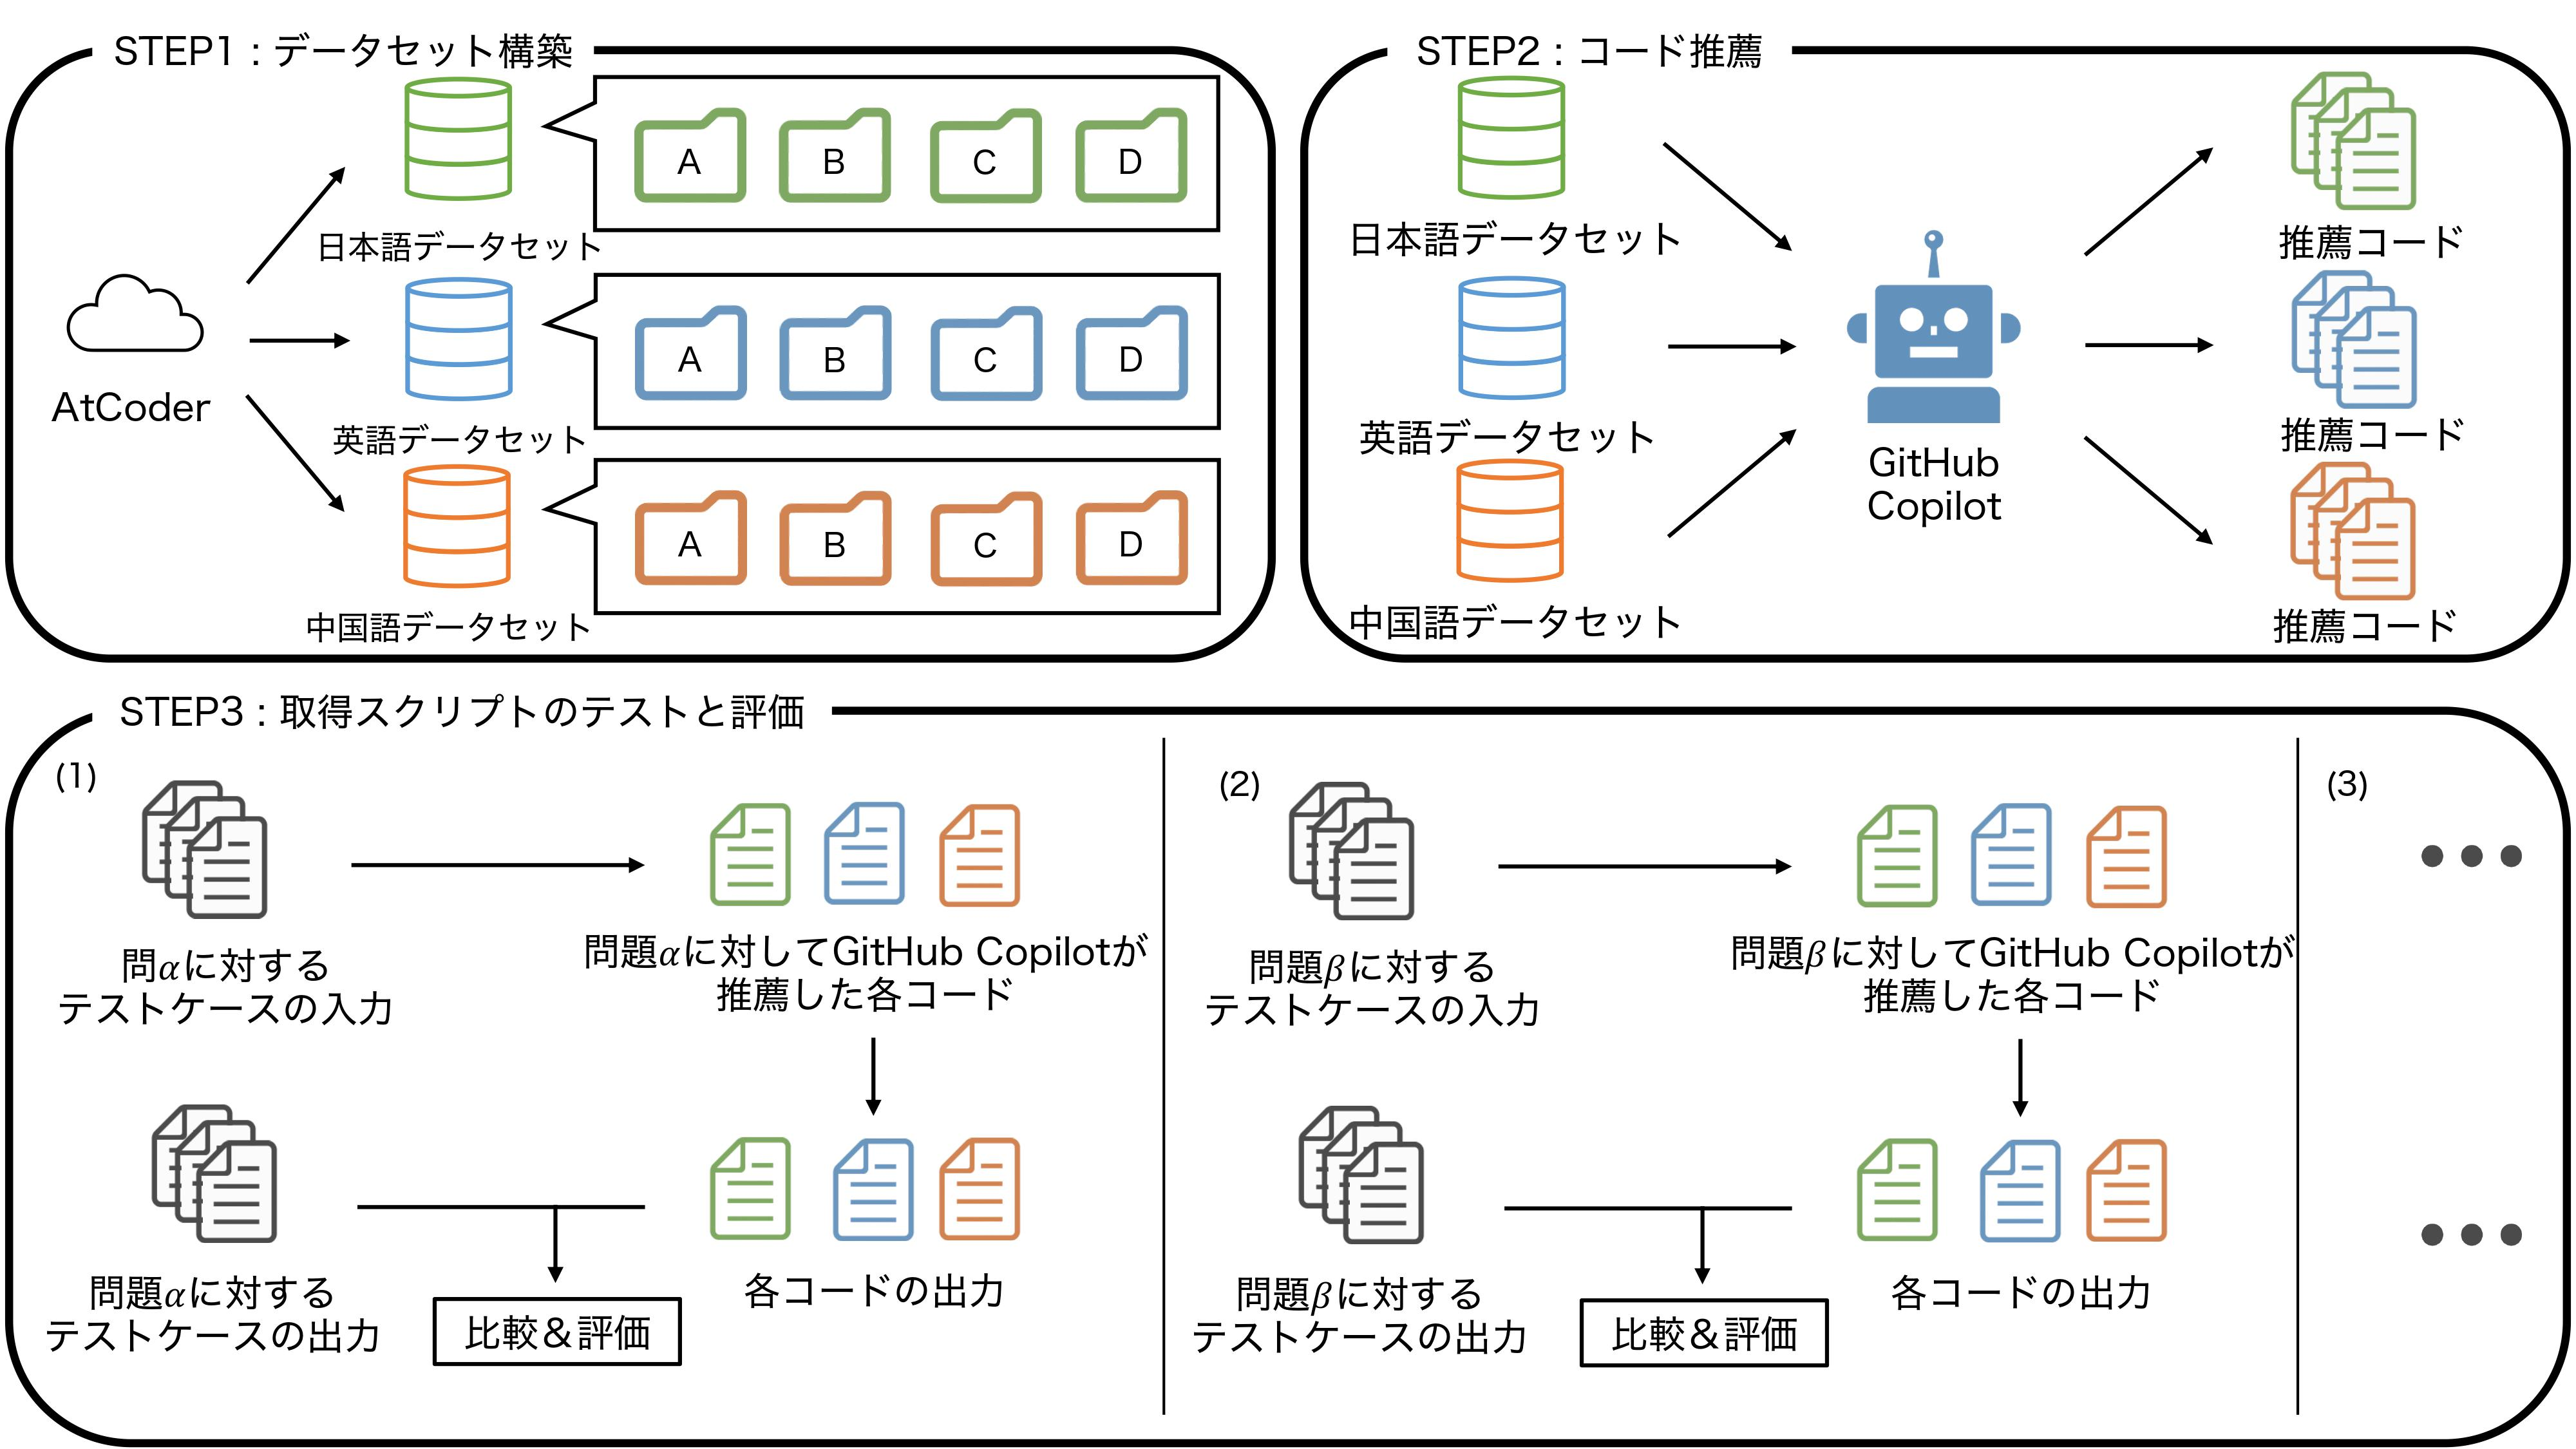
\includegraphics[scale=0.35]{image/system.jpg}
    \caption{実験設計の概要}
    \label{experiment_design}
  \end{figure*}
  
  \subsection{データセット構築\label{build_dataset}}
    本研究では日本国内において最大の競技プログラミングコンテストであるAtCoder\cite{AtCoder}の問題を使用する.
    中でも,AtCoder Beginner Contestという毎週開催されているコンテストの問題を使用する.
    
    このコンテストは開催番号1${\sim}$307(2023/06/24現在)が公開されており,
    各コンテストにはA, B, C, D, E, F, G, Ex(H)までの最大8段階の,難易度の異なる問題が存在し,
    アルファベットの語順が後になるほど難易度が高くなる.
    A問題は簡単な文法の確認,B問題は簡単な文法に加えてif文やfor文の処理,
    C問題は計算量を意識した処理,D問題はアルゴリズムを考慮した処理,
    E問題以降は複数のアルゴリズムを考慮した処理を行う問題である.
    また,問題は日本語版と英語版が準備されている.
    
    この問題の中から,開催番号99${\sim}$287,各問題の難易度A${\sim}$Dの日本語版および英語版を使用する.
    問題を限定する理由として,
    開催番号はテストケースが存在している問題を使用するため,
    問題難易度はE問題以降,複数のアルゴリズムを考慮した複雑な処理が必要となるため,
    D問題までの問題を使用する.
    
    続いて,中国語版の問題はAtCoderには存在しないため,
    英語版のデータセットをDeepL APIを使用して翻訳し,
    翻訳した問題をソフトウェア工学における研究歴が約6年ある中国人研究者によって校正することで,中国語版のデータセットを作成する.
    最終的に,開催番号が99${\sim}$287,各問題の難易度がA,B,C,D,問題の言語が英語,日本語,中国語の3つのデータセットを取得し,
    これらを本実験のデータセットとする.

\vspace{-1zh}
  \subsection{コード推薦\label{recommend_program}}
    \ref{build_dataset}節で作成したデータセットに対して,Copilotでコード推薦を行う.
    \ref{build_dataset}節で作成した各言語のデータセットの中には,開催番号が99${\sim}$287,各問題の難易度がA,B,C,D存在するため,
    合計で756問ある.
    これらの各問題に対して,それぞれコード推薦を行う.
    
    \begin{figure}[t]
      \begin{tabular}{c}
        \begin{tabularx}{23zw}{l}
          \hline
          \verb|[問題文]| \\
          \textrm{  高橋くんは A グラムの純金と B グラムの純銀} \\
          \textrm{  ($0 \leq A, B, 0 < A+B$) をよく溶かした上で} \\
          \textrm{  混ぜ合わせ、新たな金属を生成しました。} \\
          \textrm{  生成された金属は「純金」「純銀」「合金」の} \\
          \textrm{  いずれでしょうか?} \\
          \textrm{  なお、生成された金属は} \\
          \textrm{  $0 < A$ かつ $B = 0$ なら「純金」} \\
          \textrm{  $A = 0$ かつ $0 < B$ なら「純銀」} \\
          \textrm{  $0 < A$ かつ $0 < B$ なら「合金」} \\
          \textrm{  であるとみなします。} \\
          \verb|[制約]| \\
          \textrm{  $0 \leq A,B \leq 100$} \\
          \textrm{  $0 < A+B$} \\
          \textrm{  A, B は整数} \\
          \verb|[入力]| \\
          \textrm{  入力は以下の形式で標準入力から与えられる。} \\
          \textrm{  A B} \\
          \verb|[出力]| \\
          \textrm{  生成された金属が「純金」なら Gold と、} \\
          \textrm{  「純銀」なら Silver と、} \\
          \textrm{  「合金」なら Alloy と出力せよ。} \\
          \verb|[入力例 1]| \\
          \textrm{  50 50} \\
          \verb|[出力例 1]| \\
          \textrm{  Alloy} \\
          \verb|[入力例 2]| \\
          \textrm{  100 0} \\
          \verb|[出力例 2]| \\
          \textrm{  Gold} \\
          \hline
        \end{tabularx}
      \end{tabular}
      \caption{問題212-Aの日本語版}
      \label{problem_212_A_en}
    \end{figure}

    図\ref{problem_212_A_en}は問題212-Aの日本語版のデータセットの中身である\cite{AtCoder}.
    このように各問題のデータセットには,問題,制約,入力,出力,入力例,出力例がコメントとして記述されている.
    ただし,問題によって入力例および出力例の数は異なり,また注釈等の追加の記述がある場合もある.
    このデータセットを入力として,Copilotによるコード推薦を行い,$x$個の推薦コードを得る.
    このとき,$x$は$0 {\leq} x {\leq} 10$を満たす.
    また,推薦コードで出力するプログラミング言語はPythonを使用する.
    この入力から出力までの流れを各問題に対して5回実行する.
    その理由としては,Copilotの推薦コードが毎回変化するため,
    このランダム性を考慮して,評価を行うためである.
    
\vspace{-1zh}
  \subsection{取得コードのテストと評価\label{test_and_evaluation}}
    \ref{recommend_program}節で取得したコードに対して,テストを行う.
    このテストは,各問題に対してテストケースの入力を標準入力として与え,取得したコードを実行し,テストケースの出力と一致するかを確認する.
    そして,各推薦コードが全てのテストケースを通過したか否かで評価を行う.
    使用した評価指標は,$Accuracy$(正答率)で,推薦された全コードの内,全てのテストケースを通過したコードの割合を示す.
    ただし,Copilotが推薦したコードの順番は考慮せずに評価を行う.
\vspace*{-1zh}